\documentclass[12pt]{article}
\usepackage{graphicx}
\usepackage[margin=1.0in]{geometry}   % sets all margins to 1in, can be changed
\usepackage{moreverb}                 % for verbatimtabinput -- LaTeX environment
\usepackage{rotating}
\usepackage{url}     
\usepackage{hyperref}
\usepackage{multirow}
\usepackage{amssymb}                  % for many mathematical symbols
\usepackage[pdftex]{lscape}           % for landscaped tables
\usepackage{longtable}
\usepackage[dvipsnames]{xcolor}
\usepackage[spanish]{babel}
\usepackage[utf8]{inputenc}


\newtheorem{Def}{Definici\'on}[section]
\newtheorem{Ejem}{Ejemplo}[section]
\newtheorem{Teo}{Teorema}[section]
\newtheorem{Dem}{Demostraci\'on}[section]
\newtheorem{Note}{Nota}%[section]
\newtheorem{Sol}{Soluci\'on}[section]
\newtheorem{Prop}{Proposici\'on}[section]
\newtheorem{Coro}{Corolario}[section]



\title{Un primer estudio estad\'istico de la Certificaci\'on en la UACM}
\author{Carlos E. Martínez-Rodríguez\thanks{Departamento de Estadística, Universidad Autónoma de la Ciudad de México (UACM). Correo electrónico: carlos.martinez@uacm.edu.mx}}
\date{27 de noviembre de 2022}

\begin{document}
\maketitle
\tableofcontents

\section{Introducci\'on y antecedentes}


\subsection{Artículo 1: Machine Learning in Enzyme Engineering}
Título: \href{https://pubs.acs.org/doi/full/10.1021/acscatal.9b04321}{Machine Learning in Enzyme Engineering, Stanislav Mazurenko, Zbynek Prokop, and Jiri Damborsky} \cite{Mazurenko}

\begin{itemize}
\item Enzyme engineering is the process of customizing new biocatalysts with improved properties by altering their constituting sequences of amino acids.

\item Multiple ML algorithms have already been applied to enzyme engineering. Some notable examples include random forests used to predict protein solubility \cite{15}, support vector machines \cite{16},\cite{17} and decision trees \cite{18} to predict enzyme stability changes upon mutations, K-nearest-neighbor classifiers to predict enzyme function\cite{19} and mechanisms,\cite{20} and various scoring and clustering algorithms for rapid functional sequence annotation \cite{21},\cite{22}. The main attractiveness of ML in enzyme engineering stems from its generalizability: once it is trained on the known input, called a training set, an ML algorithm can potentially make predictions about new variants almost instantly.

\item The aim of this Perspective is, therefore, to highlight recent advances in data collection and algorithm implementation for ML in enzyme engineering. 

\end{itemize}

\subsection{The essence of Machine Learning}

La esencia de la mayoría de los algoritmos de Machine Learning (ML) es encontrar patrones en los datos disponibles, datos que consisten en varios descriptores o características, por ejemplo secuencias de encimas, sus estructuras secundarias y terciarias, substiruciones, etc.  El nímero de características usualmente varían de decenas a miles lo que convierte el problema en uno de alta dimensión. 

\begin{figure}{ht!}
\centering
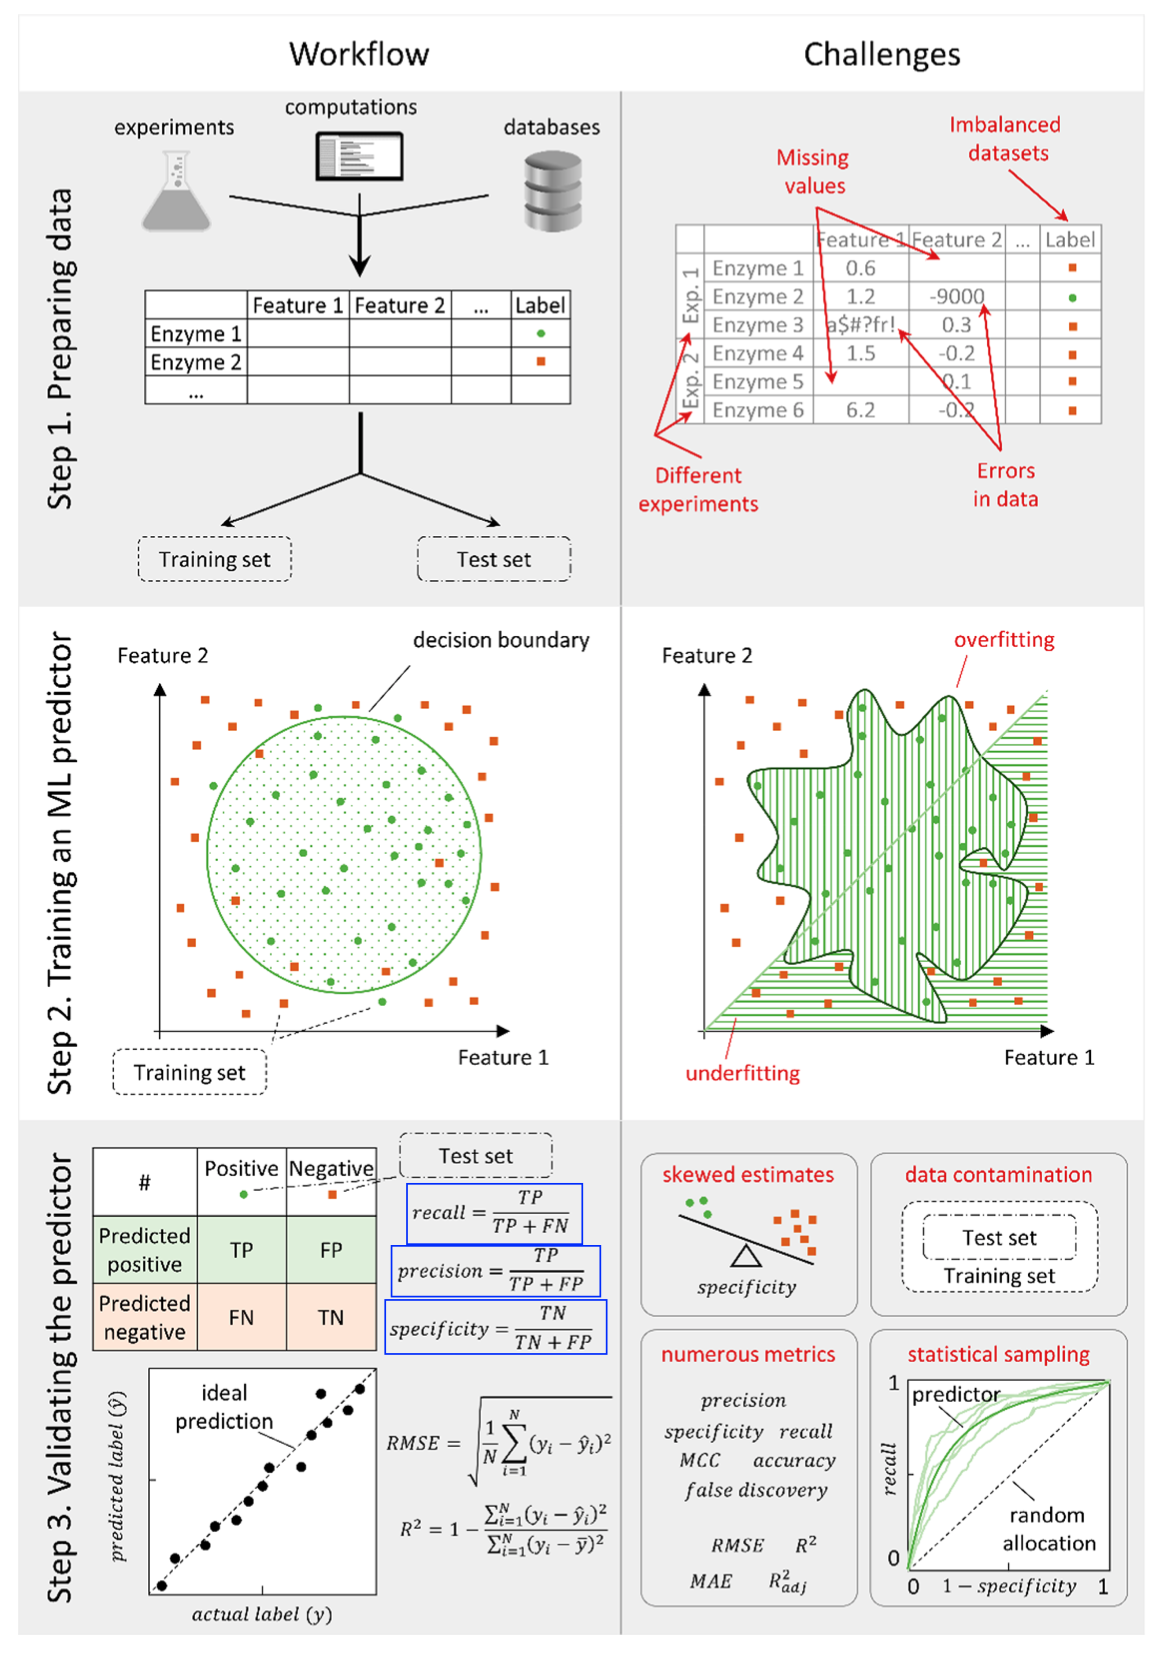
\includegraphics[scale=0.45]{Figura2.png}
\caption{Schematic workflow of constructing an ML predictor and associated challenges. }
\label{Figura2}
\end{figure}

Los principales tipos de Machine Learning son: Aprendizaje Supervisado y Aprendizaja No-Supervisado. En el aprensizaje no supervisado el objetivo es disminuir la alta dimensionalidad de los datos en uno de menor dimensión, o el de encontrar clústers en los datos.  En el aprendizaje supervisado varias propiedades objetivo tales como actividad o estabilidad de enzimas,  y el objetivo es diseñar un predictor que regrese etiquetas para datos no vistos considerando sus descriptores,  utilizando el conjunto de datos etiquetado como datos de entrenamiento.

\begin{Note}
Step 1: the data are usually turned into a table format and split into the training and test parts. Any errors, biases, or imbalances will be translated to the predictor’s performance and, hence, must be accounted for. Step 2: the predictor is trained on the training data set. For example, a decision boundary is derived that allows classifying future input based on whether data points are inside or outside the boundary. This is a balancing act between two extremes: explaining noise rather than fundamental dependencies (overfitting) or failure to account for complex dependencies in the data (underfitting). Step 3: the performance of the predictor is evaluated based on the test data set. For example, true and false positives and negatives and the associated measures are calculated or the root mean square error (RMSE) is calculated for continuous labels. The random nature of the initial data split as well as data imbalances might skew the evaluation, and numerous metrics used for evaluation vary in their robustness to different data skews. Even partial inclusion of the test set at any stage of ML predictor training is called data contamination and usually invalidates the final evaluation.

\end{Note}

\section{Artículo 2: }



\section{Referencias}

\begin{thebibliography}{20}
\bibitem{Mazurenko}Mazurenko, S., Prokop, Z., and Damborsky, J. (2019). Machine learning in enzyme engineering. ACS Catalysis, 10(2), 1210-1223. 

\bibitem{15} Yang, Y.; Niroula, A.; Shen, B.; Vihinen, M. PON-Sol: Prediction of Effects of Amino Acid Substitutions on Protein Solubility. Bioinformatics 2016, 32, 2032!2034.

\bibitem{16} Folkman, L.; Stantic, B.; Sattar, A.; Zhou, Y. EASE-MM: Sequence-Based Prediction of Mutation-Induced Stability Changes with Feature-Based Multiple Models. J. Mol. Biol. 2016, 428, 1394! 1405.

\bibitem{17} Teng, S.; Srivastava, A. K.; Wang, L. Sequence Feature-Based Prediction of Protein Stability Changes upon Amino Acid Substitutions. BMC Genomics 2010, 11, S5.

\bibitem{18} Huang, L.; Gromiha, M. M.; Ho, S. iPTREE-STAB: Interpretable Decision Tree Based Method for Predicting Protein Stability Changes Upon Mutations. Bioinformatics 2007, 23, 1292! 1293.


\bibitem{19} Koskinen, P.; Toronen, P.; Nokso-Koivisto, J.; Holm, L. PANNZER: High-Throughput Functional Annotation of Uncharac- terized Proteins in an Error-Prone Environment. Bioinformatics 2015, 31, 1544!1552.

\bibitem{20} De Ferrari, L.; Mitchell, J. B. From Sequence to Enzyme Mechanism Using Multi-Label Machine Learning. BMC Bioinf. 2014, 15, 150.

\bibitem{21} Falda, M.; Toppo, S.; Pescarolo, A.; Lavezzo, E.; Di Camillo, B.; Facchinetti, A.; Cilia, E.; Velasco, R.; Fontana, P. Argot2: A Large Scale Function Prediction Tool Relying on Semantic Similarity of Weighted Gene Ontology Terms. BMC Bioinf. 2012, 13, S14.

\bibitem{22} Cozzetto, D.; Buchan, D. W.; Bryson, K.; Jones, D. T. Protein Function Prediction by Massive Integration of Evolutionary Analyses and Multiple Data Sources. BMC Bioinf. 2013, 14, S1.


\end{thebibliography}


\end{document}